\RequirePackage{fix-cm}
\documentclass[twocolumn]{svjour3}
% Springer svjour3 template (same as used by the course).
% STAGE: first vision of the publication (Z6). Blue text = planned content / bullet points,
% to be turned into prose for draft 1. Red text in brackets = open decisions.

\usepackage{cite}
\usepackage{graphicx}
\usepackage{amsmath}
\usepackage{amssymb}
\usepackage{xcolor}
\usepackage{booktabs}
\usepackage{multirow}
\usepackage{url}
\usepackage{balance}
\usepackage{placeins}

\newcommand{\plan}[1]{{\color{blue!70!black}#1}}   % planned content, to become prose
\newcommand{\open}[1]{\textcolor{red!70!black}{[#1]}} % open decision for the authors
\graphicspath{{figs/}}

\journalname{\open{Target venue: to decide}}

\begin{document}

\title{Two Questions Are Enough: Budgeted User Questions for Calorie Estimation from Meal Photos}
\titlerunning{Budgeted user questions for photo-based calorie estimation}

\author{Adam~Soko{\l}owski \and Antoni~Grajek}
\authorrunning{A.~Soko{\l}owski, A.~Grajek}

\institute{A.~Soko{\l}owski, A.~Grajek \at
  Warsaw University of Technology, \open{faculty / institute to confirm}
}

\date{Received: date / Accepted: date}

\maketitle

\begin{abstract}
% Draft written with the Dunleavy scheme (context / difference / method / results / one thing to remember).
% It will be rewritten last, after the whole paper is done.
Vision-language models can estimate the energy content of a meal from a single photo, but they miss
portion size and hidden ingredients, and their errors stay large. Recent interactive systems close part
of this gap by asking the user, yet they ask many questions and assume the user knows the exact answer.
We study the realistic setting in which an application may ask at most three questions and people answer
with error. On 424 test dishes from Nutrition5k we evaluated an open model (Qwen2.5-VL-7B) with a pool of
seven questions, four simulated users (ideal, noisy grams, category mistakes, ``don't know'') and five
question-selection strategies, including a learned uncertainty-driven selector. Two well-chosen questions
recovered 84\% of the error reduction obtained by asking all seven (mean absolute percentage error 52.8\%
$\rightarrow$ 43.9\% vs.\ 42.2\%). The learned selector beat random choice and a model that chose its
own questions, but not a fixed question order. Asking for the portion category was more useful than asking
for grams, whose value dropped by 37\% under realistic noise, while asking for an ingredient list or about
added fat increased the error. A short, fixed questionnaire about portion size is therefore a strong and
simple default for calorie-tracking applications.
\keywords{calorie estimation \and vision-language models \and clarifying questions \and active feature acquisition \and Nutrition5k}
\end{abstract}

% =====================================================================
\section*{Publication vision (Z6; this box is removed in draft 1)}
\label{sec:vision}

\paragraph{Model reader.}
Researchers building food-logging and dietary-assessment tools with multimodal models (computer vision
for nutrition, mHealth), and readers from the active feature acquisition / clarifying-questions community.
They know what a VLM is; they do not know Nutrition5k details or human portion-estimation error.

\paragraph{Main message (the glue of the paper).}
\emph{With a budget of 1--3 questions and realistic answers, \textbf{which} questions you ask matters
more than \textbf{how cleverly} you choose them: two questions about portion size give most of the
gain, a fixed order is as good as a learned selector, and some ``natural'' questions hurt.}

\paragraph{Title candidates} (max.\ 15 words, no acronyms; to choose):
\begin{enumerate}
  \item Two Questions Are Enough: Budgeted User Questions for Calorie Estimation from Meal Photos
  \item How Many Questions Are Enough? Asking About a Meal When Users Answer Imprecisely
  \item Ask About Portion Size, Not Ingredients: Budgeted Questions for Photo-Based Calorie Estimation
\end{enumerate}

\paragraph{Structure.} IMRaD, two columns, about 8--10 pages: Introduction (with a short related-work
part), Methods (data, questions, simulated users, model, strategies, metrics), Results (budget, strategies,
noise, question ranking, subgroups), Discussion (interpretation, practical recommendations, limitations,
future work), Conclusions.

\paragraph{Style.} English, past tense in Methods and Results, present tense for general statements.
Paragraphs follow the topic sentence -- concrete detail -- commentary -- closing sentence scheme.
Negative results (H2 vs.\ fixed order, H4) are reported plainly, not hidden.

\paragraph{Missing material} (no new GPU runs are planned):
\begin{itemize}
  \item Verify six references marked ``to verify'' in the literature review (CalorieLLaVA, CalorieVoL,
        ViT nutrient values, prompt engineering 2026, information-gain clarification, the 2024 study on
        over-/under-estimation).
  \item Two small analyses from the existing cache (CPU only): (a) significance on MAE and acc@20\%,
        where S4 looks better than S2 although MAPE does not differ; (b) how often the per-dish best
        question differs from the fixed order (headroom of the oracle).
  \item One method figure (pipeline: photo $\rightarrow$ question selection $\rightarrow$ simulated
        answer $\rightarrow$ VLM $\rightarrow$ estimate).
  \item Descriptive statistics of the test set (kcal, mass, number of ingredients, fat share).
\end{itemize}

\paragraph{Schedule.}
\begin{tabular}{@{}ll@{}}
  Z6 (now)       & this vision + presentation \\
  Draft 1        & full Introduction, Methods, Results; Discussion in bullets \\
  Draft 2        & complete paper: Discussion, Conclusions, abstract \\
  Final (25.01)  & revisions after discussions, final slides \\
\end{tabular}
\open{Exact dates of the two draft discussions: to confirm with the supervisor.}

% =====================================================================
\section{Introduction}
\label{sec:intro}
\plan{
\textbf{Context.} Diet tracking apps increasingly estimate calories from a photo; general-purpose VLMs
can do it zero-shot. \textbf{What is known.} Errors remain large: RGB models on Nutrition5k reach
14--26\% calorie error~\cite{thames2021nutrition5k,han2023dpf}, zero-shot VLMs 35--55\%
MAPE~\cite{fridolfsson2025llm,bhatambarekar2025thesis}; portion size and hidden fats are the main
sources~\cite{lo2020review,vinod2026portion,nutrients2026prompt}. Extra information from the user helps:
ingredient masses lower GPT-4o MAPE from about 51\% to 29\%~\cite{bhatambarekar2025thesis}, metadata
helps~\cite{coburn2025lmm}, an agent asking its own questions helps~\cite{bhatambarekar2026agentic}.
\textbf{What is not known.} (1) No question budget: prior work asks everything or without limit, while
every question adds user burden~\cite{hochsmann2020review}. (2) Answers are taken from ground truth,
while people estimate portions poorly (35--50\% of answers within $\pm$25\%)~\cite{lucassen2021portion}.
(3) Active feature acquisition and information-gain question selection~\cite{aronsson2025afa,kobalczyk2025active}
have not been applied here. \textbf{Research questions} RQ1--RQ3 and hypotheses H1--H4 (from
\texttt{docs/01}, \texttt{docs/03}). \textbf{Contributions:} evaluation protocol with a budget and
calibrated simulated users; error-vs-budget curves and strategy comparison; recommendations which
questions to ask real users. Related work either as the last part of the Introduction or a short
Section~2 \open{(to decide)}.
}

% =====================================================================
\section{Methods}
\label{sec:methods}

\subsection{Data}
\plan{Nutrition5k~\cite{thames2021nutrition5k}: overhead RGB photos, weighed ingredients. Validation:
300 dishes sampled from the official train split (seeded); test: official test split. Dishes under
50\,kcal removed (percentage error explodes on near-empty plates): 300 validation, 424 test dishes.
True answers to all questions derived from metadata (fat and sauce lexicons, mass terciles from
validation: $<$153\,g, 153--288\,g, $>$288\,g). Table of dataset statistics \open{(to add)}.}

\subsection{Question pool}
\plan{Seven questions: Q1 mass in grams, Q2 small/medium/large, Q3 fried or oil/butter, Q4 sauce or
dressing, Q5 main ingredient, Q6 list of ingredients, Q7 number of items. Answers enter the prompt as
a list of facts, so a set of questions defines the prompt independently of their order. Table: question,
answer type, source in Nutrition5k.}

\subsection{Simulated users}
\plan{U0 ideal; U1 log-normal mass error $m' = m\,e^{\varepsilon}$, $\varepsilon\sim\mathcal{N}(\mu,\sigma)$,
$\sigma\in\{0.1, 0.33, 0.5\}$, bias $\mu=0.2$, calibrated on~\cite{lucassen2021portion}; Q2 uses the same
perceived mass (consistent user); U2 category mistakes with $p\in\{0.1,0.2\}$; U3 ``don't know'' with
$q=0.2$ (budget spent). Answers drawn once per dish and user, so a user is consistent across question sets.}

\subsection{Model and prompt}
\plan{Qwen2.5-VL-7B-Instruct (AWQ 4-bit) served with vLLM, temperature 0, JSON output
\{kcal, mass\_g, confidence\}; no chain of thought (pilot: slower and worse). 0\% parse failures.
Key trick: predictions precomputed for all $1+7+21+35=64$ question subsets of size $\le 3$ and every user
variant (about 112k unique calls, about 36\,h on one laptop GPU); every strategy except S3 is then
evaluated offline.}

\subsection{Question-selection strategies}
\plan{S0 photo only; S1 random (expectation over subsets); S2 fixed greedy order learned on validation;
S3 the VLM picks the next question itself (online, U0 and U1); S4 ours: LightGBM predicts the error
reduction of each candidate question from uncertainty features (spread of $K=5$ samples at temperature 0.7,
stated confidence), the current estimate and answers so far, greedy step by step; oracle: best subset per
dish chosen with ground truth (upper bound).}

\subsection{Metrics and statistics}
\plan{MAPE (main), MAE, acc@20\%; share of oracle gain; gain recovered relative to all seven questions.
Paired Wilcoxon test on per-dish errors, bootstrap 95\% CI, Holm correction per user variant.}

% =====================================================================
\section{Results}
\label{sec:results}
\plan{Order follows the research questions. Objective description only; interpretation goes to the
Discussion.}

\subsection{Error versus number of questions (RQ1, H1)}
\plan{Photo only 52.8\% MAPE; all seven questions 42.2\%. Two questions (S4) 43.9\%, i.e.\ 84\% of the
full-information gain (H1 threshold 70\%: met). Third question adds little (42.7\%). The oracle reaches
24.6\% at $B=2$; S4 obtains 32\% of the oracle's gain. Fig.~\ref{fig:budget}, Table~\ref{tab:main}.}

\begin{figure*}[t]
  \centering
  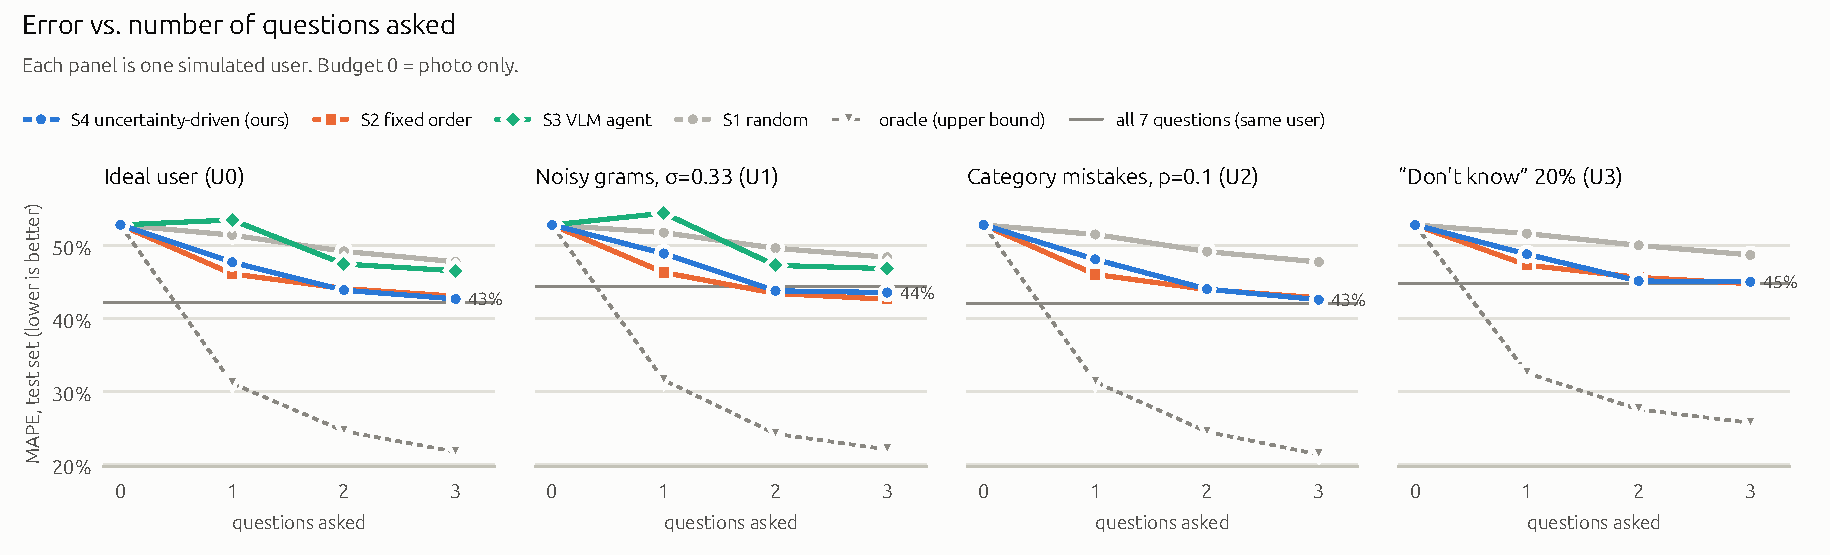
\includegraphics[width=\textwidth]{fig1_budget_curves}
  \caption{Calorie error (MAPE, test set) versus the number of questions asked, for four simulated users.
  Budget 0 is the photo only; the horizontal line is the error with all seven questions.}
  \label{fig:budget}
\end{figure*}

\begin{table}[t]
  \centering
  \caption{MAPE [\%] on the test set ($n=424$). Photo only: 52.8\%. All seven questions: 42.2\% (U0),
  44.4\% (U1).}
  \label{tab:main}
  \setlength{\tabcolsep}{3.5pt}
  \begin{tabular}{@{}llrrrrr@{}}
    \toprule
    User & $B$ & S1 & S2 & S3 & S4 & Oracle \\
    \midrule
    \multirow{3}{*}{U0 ideal}        & 1 & 51.4 & 46.1 & 53.5 & 47.7 & 31.1 \\
                                     & 2 & 49.2 & 44.1 & 47.5 & 43.9 & 24.6 \\
                                     & 3 & 47.8 & 43.1 & 46.5 & 42.7 & 21.7 \\
    \midrule
    \multirow{3}{*}{U1 $\sigma{=}0.33$} & 1 & 51.8 & 46.3 & 54.5 & 48.9 & 31.6 \\
                                     & 2 & 49.6 & 43.5 & 47.3 & 43.8 & 24.2 \\
                                     & 3 & 48.4 & 42.6 & 46.8 & 43.6 & 22.0 \\
    \bottomrule
  \end{tabular}
\end{table}

\subsection{Comparison of strategies (RQ2, H2)}
\plan{S4 significantly better than random for every user at $B\in\{1,2\}$ ($p_{\text{Holm}}\le 0.03$) and
better than the VLM agent for U0 and U1. No significant difference between S4 and the fixed order S2
(differences $-2.5$ to $+2.6$\,pp, CIs contain zero): H2 partially supported. The VLM agent at $B=1$ is worse
than the photo alone; it picks the ingredient list (Q6) for 36\% of dishes. Table of test results with CIs
\open{(to add)}. Additional: S4 has lower MAE and higher acc@20\% than S2 (\open{significance to check}).}

\subsection{Effect of noisy answers and question ranking (RQ3, H3)}
\plan{The gain of the grams question drops by 37\% under U1 (5.9 $\rightarrow$ 3.7\,pp; threshold 30\%:
met). The portion category (Q2) is then better than grams (6.5 vs.\ 3.7\,pp), but it is already the best
question for the ideal user, so the ranking does not change: Q2 $>$ Q1 $>$ Q4 $>$ Q7 $>$ Q5 $>$ Q3 $>$ Q6.
The ingredient list (Q6) increases error by about 7\,pp for every user. Fig.~\ref{fig:ranking}.}

\begin{figure*}[t]
  \centering
  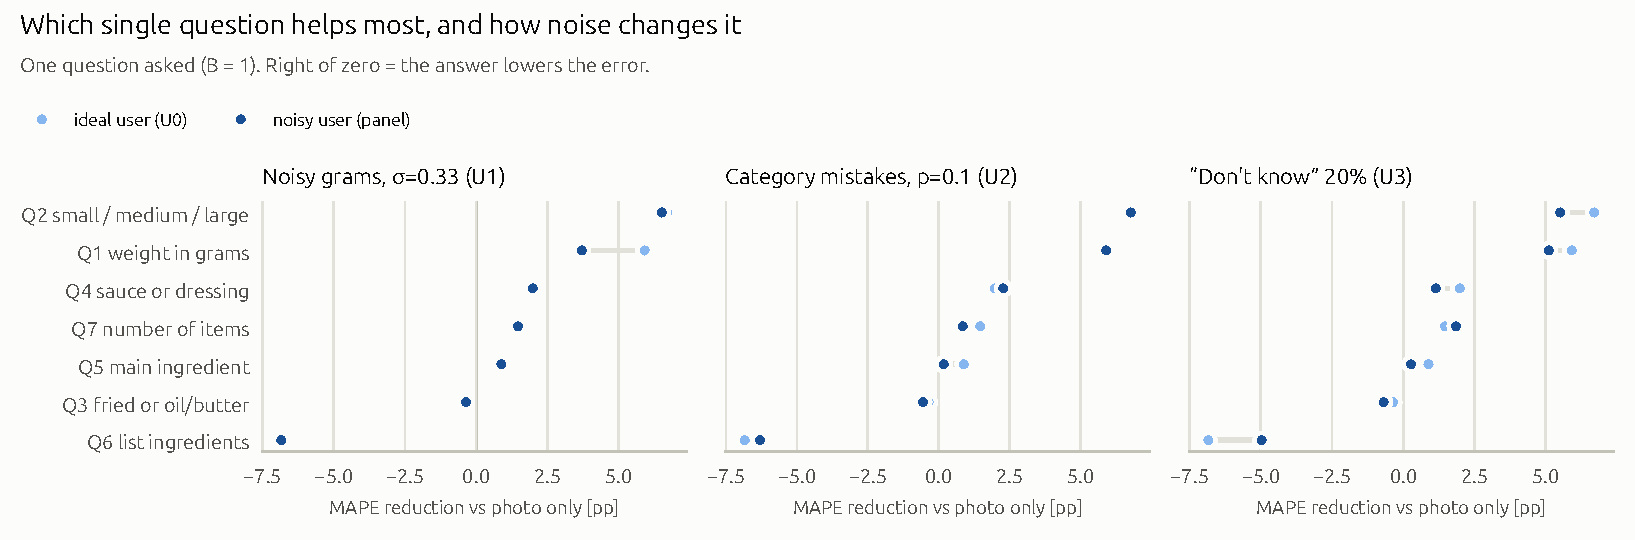
\includegraphics[width=\textwidth]{fig2_question_ranking}
  \caption{MAPE reduction of each single question (one question asked) for the ideal user and three
  noisy users.}
  \label{fig:ranking}
\end{figure*}

\subsection{Subgroups (H4)}
\plan{For fat-heavy dishes ($>$30\% of kcal from fat, $n=297$) the fat question Q3 increases error
($-3.2$\,pp) and Q2 is best (5.6\,pp); Q3 helps only lean dishes (+6.2\,pp): H4 not supported. Q2 helps
small portions strongly (+20.6\,pp) and large portions not at all. Fig.~\ref{fig:subgroups}.}

\begin{figure}[t]
  \centering
  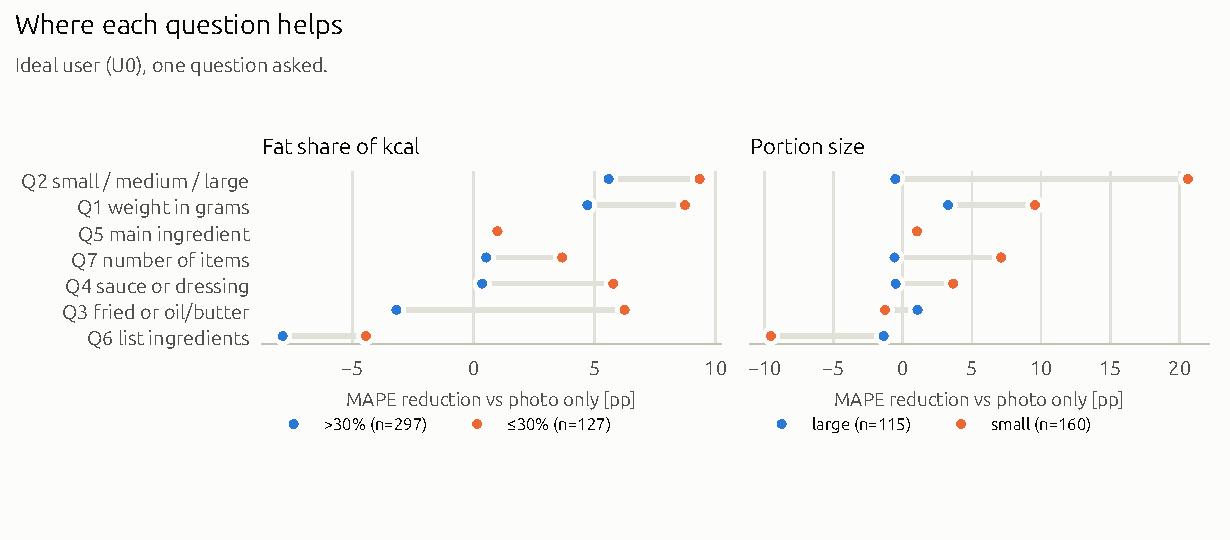
\includegraphics[width=\columnwidth]{fig3_subgroups_U0}
  \caption{Single-question gain in subgroups (ideal user): fat share of energy and portion size.}
  \label{fig:subgroups}
\end{figure}

% =====================================================================
\section{Discussion}
\label{sec:discussion}
\plan{
\textbf{Answer to RQ1:} two questions are enough; diminishing returns after that.
\textbf{Why a learned selector does not beat a fixed order:} the model's sampling spread carries almost no
signal (in 95\% of dishes all five samples are identical), so the selector has little to condition on;
its most important features are the candidate question and the current estimate. This is consistent with
LLMs being poor sequential planners~\cite{perets2026zeroshot} and with the agent result in
\cite{bhatambarekar2026agentic} only partly. \textbf{Headroom:} the oracle (24.6\%) shows that per-dish
selection could pay off if a better uncertainty signal existed (paraphrase ensembles, token
probabilities). \textbf{Why some questions hurt:} the ingredient list and the fat answer seem to make the
model over-correct upwards. \textbf{Practical recommendations} for apps: ask for the portion category, then
the main ingredient; avoid grams and ingredient lists. \textbf{Limitations:} one model, 4-bit quantised;
simulated users calibrated from literature, not from our own study; Nutrition5k is cafeteria food from
one place; MAPE sensitive to small dishes (50\,kcal threshold). \textbf{Future work:} second VLM, study
with real users, better uncertainty estimates.
}

% =====================================================================
\section{Conclusions}
\label{sec:conclusions}
\plan{Answer RQ1--RQ3 in three sentences; one-sentence recommendation; one sentence on future work.}

\section*{Statements and Declarations}
The authors declare that no funds, grants, or other support were received during the preparation of this
manuscript. The authors have no relevant financial or non-financial interests to disclose. Code and
results are available at \url{https://github.com/Qasdfyk/how-many-questions}.

\balance
\bibliographystyle{spmpsci}
\bibliography{references}

\end{document}
